Note that graph $G = (V,E)$ describes a social network with $V$ denoting the set of nodes and $E$ the set of edges. Further, $|V| = n$, $|E| = m$ and $u,v$ are nodes of G. The set of neighbors of $u$ is denoted by $N(u)$ and the degree of node $u$ by $d_u=|N(u)|$. We will always assume $d_u \geq 1  \forall u$. Additionally, $f : V \rightarrow \{0,1\}$ is a binary function which takes a node as input and outputs whether this node satisfies a certain property or not and $\bar{f} = \frac{1}{n}|\{u\;|\;f(u) = 1\}|$ is the fraction we wish to estimate.
The algorithms use $S$ as the set of nodes called "sample" with $|S| = r$ (sample size).

Our goal is to estimate the portion of nodes $v \in C$ such that $f(v) = 1$.
We introduce the concept of a set of algorithms called sampler which is defined as follows:
\begin{definition}[sampler]
  A sampler $\hat{f}(n,\epsilon,\delta)$ is a randomized algorithm with input $r$ (sample size), $\epsilon$ (sampler accuracy), $\delta$ (sampler error) and function $f$ which outputs $\hat{f}=\frac{1}{r}\sum\nolimits_{u\in S} f(u)$ with probability $1-\delta$ and $|\hat{f}-\bar{f}<\epsilon|$. Namely,
  $$\textbf{Pr}[|\hat{f}(n,\epsilon,\delta)-\bar{f} | > \epsilon] < \delta$$
\end{definition}

Note, that this definition of a sampler is covered in the definition of a statistical estimator.
Therefore we can analyze our sampler for estimator properties like bias and we will use both expressions equivalently.

We will start by looking at an intuitive approach for estimating $\bar{f}$ where we sample a set of nodes and poll each node $u$ to test if $f(u)=1$.
The algorithm will return the fraction of nodes that satisfy the condition and we call this approach the \texttt{Naive} estimator \cite{goldreich1997sample}.

%---algo1----------------------------------------------
\begin{algorithm*}[!htb]
  \caption{\small {\bf Naive size estimator}($G, f, r$)}
  \begin{code}
  {\bf Input:} Graph $G=(V,E)$, function $f : V \rightarrow \{0,1\}$, sample size $r$ \\
  {\bf Output:} $\hat{f}=\frac{1}{r}\sum\nolimits_{u\in S} f(u)$\\
  \\
  \uln \>\ubegin\\
  \uln \>\>initialize $f^*$ with 0 \\
  \uln \>\>randomly draw a set $S$ with r samples from $V$ with replacement\\
  \uln \>\>\ufor each element $u \subset S$ \udo\\
  \uln \>\>\>$f^* = f^* + f(u)$ \\
  \uln \>\>\uend\\
  \uln \>\ureturn $\hat{f} = f^*/r$ \\
  \uln \>\uend\\ 
  \end{code}
  \label{alg:main}
\end{algorithm*}
%---end algo2------------------------------------------
Note that in practice the drawing can be done by simply including a node $u$ with probability $\frac{1}{n}$.
\begin{theorem}
  The \texttt{Naive} estimator with accuracy $\epsilon$ and confidence $1-\delta$ requires $O(\frac{1}{\epsilon^2})$ sample nodes
\end{theorem}
\textbf{\textit{Proof: }}Recall that we want to poll $r$ uniformly chosen people independently and with replacement. The true fraction we want to approximate is $\bar{f}$. Let $F_u$ be the random variable for $f(u) = 1$.

It follows that $F_u \sim  Bernoulli(\bar{f})$ and $F_1, F_2, \ldots , F_r$ are independent.
Let $F_1, F_2, \ldots , F_r$ and $\hat{F} = X/r$ (our estimator).
We want our estimate to have accuracy $\epsilon$ and confidence $1-\delta$:
$$\textbf{Pr}[|\hat{F}-\bar{f} | \leq \epsilon] \quad\geq\quad 1-\delta$$
Since $F \sim Binomial(r,\bar{f})$, $\textbf{E}[F] = r\bar{f}$ follows by definition.
Using the Chernoff Bounds the following inequality holds for any $\gamma \geq 0$
$$\textbf{Pr}[|F-r\bar{f}|\geq \gamma r\bar{f}] \quad\leq\quad 2\exp(-\frac{\gamma^2}{2+\gamma}\cdot r\bar{f})$$
$$\Leftrightarrow\quad \textbf{Pr}[|\hat{F}-\bar{f}|\geq \bar{f}\gamma] \quad\leq\quad 2\exp(-\frac{\gamma^2}{2+\gamma}\cdot r\bar{f})$$
To achieve $\hat{F}$ bounded by $\epsilon$ we set $\epsilon = \gamma\bar{f}$, so $\gamma = \epsilon/\bar{f}$. Inserted in the formula above:
$$\textbf{Pr}[|\hat{F}-\bar{f}| \geq \epsilon] \quad\leq\quad 2\exp (-\frac{\epsilon^2/\bar{f}^2}{2+\epsilon/\bar{f}}\cdot r\bar{f}) \quad=\quad 2\exp(-\frac{\epsilon^2}{2\bar{f}+\epsilon}\cdot r)$$
Since the largest possible value of $\bar{f}$ is 1, because all nodes $u$ have $f(u) = 1$, the term in $\exp(\cdot)$ is an upper bound
$$\frac{\epsilon^2}{2\bar{f}+\epsilon} \quad\geq\quad \frac{\epsilon^2}{2+\epsilon}$$
and therefore
$$\textbf{Pr}[|\hat{F}-\bar{f}| \geq \epsilon] \quad\leq\quad 2\exp(-\frac{\epsilon^2}{2+\epsilon}\cdot r)$$
Remember we want the confidence of the estimator bounded by $1-\delta$, this means
$$2\exp(-\frac{\epsilon^2}{2+\epsilon}\cdot r) \leq \delta$$
$$\Leftrightarrow\quad \exp(\frac{\epsilon^2}{2+\epsilon}\cdot r) \quad\geq\quad \frac{2}{\delta}$$
$$\Leftrightarrow\quad \frac{\epsilon^2}{2+\epsilon}\cdot r \quad\geq\quad \ln\frac{2}{\delta}$$
$$\Leftrightarrow\quad r \quad\geq\quad \frac{2+\epsilon}{\epsilon^2}\ln\frac{2}{\delta}$$
Since $\frac{2+\epsilon}{\epsilon^2}\ln\frac{2}{\delta}$ lies within $O(\epsilon^2)$ this concludes the proof.$\hfill\square$
% We set the sample size $r = \frac{ln(2/\gamma)}{2\epsilon^2}$ and consider the set of nodes $S$ with elements $u$ being drawn independently and uniformly distributed.
% Using the Chernoff Bound the following inequality holds:
% $$P[$$ 
\newline\newline
As briefly mentioned in the introduction the network structure is of great importance to the sampling method.
We will illustrate this on a small example. Consider a graph structure as shown in \rfig{network_a} where a single \texttt{RED} node is connected to several \texttt{BLUE} nodes.
Even though the portion of \texttt{RED} nodes is way smaller, using the \texttt{Naive} estimator the result is very biased towards the decision of {RED}.

To circumvent this behaviour we introduce an improved sampler called \texttt{Ideal} estimator that divides each $f(v)$ by $d_v$. The pseudocode is shown below:
%---algo2----------------------------------------------
% \begin{algorithm*}[!htb]
% \caption{\small {\bf Ideal size estimator}($G, f, r$)}
% \begin{code}
% {\bf Input:} Graph $G=(V,E)$, function $f : V \rightarrow \{0,1\}$, sample size $r$, distribution $p$ \\
% {\bf Output:} $\hat{f}=\frac{1}{r}\sum\nolimits_{u\in S} f(u)$\\
% \\
% \uln \>\ubegin\\
% \uln \>\>initialize $f^*$ with 0 \\
% \uln \>\>randomly draw a set $S$ with r samples from $V$ with replacement\\
% \uln \>\>\ufor each element $u \subset S$ \udo\\
% \uln \>\>\>$f^* = f^* + f(u)$ \\
% \uln \>\>\uend\\
% \uln \>\ureturn $\hat{f} = f^*/r$ \\
% \uln \>\uend\\ 
% \end{code}
% \label{alg:main}
% \end{algorithm*}
%---end algo2------------------------------------------

%---figure network a------------------------------------
\begin{figure}
  \begin{center}
    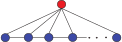
\includegraphics{fig1a}
    \caption{neighbor scaling}
    \label{fig:}
    \lfig{network_a}
  \end{center}
\end{figure}
%---end figure network a--------------------------------
